% ******************************************************** %
% DOCUMENT INFORMATION                                     %
% ******************************************************** %
%                                                          %
%                                                          %
% Purpose of Document                                      %
% -------------------                                      %
% Technical Report                                         %
%                                                          %
% Institution                                              %
% -----------                                              %
% University of Applied Sciences and Arts Northwestern     %
% Switzerland, School of Engineering                       %
%                                                          %
% Degree Program                                           %
% --------------                                           %
% Electrical Engineering and Information Technology, BSc.  %
%                                                          %
% Course                                                   %
% ------                                                   %
% Project 4, Spring Semester 2016                          %
%                                                          %
% Authors                                                  %
% -------                                                  %
% Marcel Heymann     (Firmware)                            %
% Noah Hüsser        (Hardware, Firmware)                  %
% Raphael Frey       (Simulations, Reporting)              %
% Dominik Keller     (Hardware, Firmware)                  %
% Marco Koch         (Deputy Team Leader, Simulations)     %
% Reto Nussbaumer    (Team Leader)                         %
% Francesco Rovelli  (Hardware, Firmware)                  %
%                                                          %
% Document Design and Maintenance                          %
% -------------------------------                          %
% Raphael Frey                                             %
% Based on my own work. The  template on which this report %
% was based is available at:                               %
% https://github.com/alpenwasser/longtex                   %
% -------------------------------------------------------- %

\documentclass[11pt, a4paper, oneside]{memoir}

% -------------------------------------------------------- %
% Different font and pages  sizes, layouts. Not a complete %
% list, just what I've used on occasion.                   %
% -------------------------------------------------------- %
%\documentclass[9pt,b5paper]{memoir}
%\documentclass[twocolumn,9pt,a4paper]{memoir}
%\documentclass[10pt,a5paper]{memoir} % ~60 chars per line
%\documentclass[12pt,a4paper]{memoir} % ~60 to 70 chars per line


% -------------------------------------------------------- %
% Preamble  stuff  is  kept in  the  preamble/  directory, %
% separated  out into  different files  as needed  to keep %
% things modular.                                          %
% -------------------------------------------------------- %
% -------------------------------------------------------- %
% NOTE: There   are  two   kinds  of   packages  in   this %
% document. On ond hand, there  are those which are needed %
% for this  template to function at  as intended. It might %
% still  compile without  them,  but it  will probably  no %
% longer look as it should.                                %
%                                                          %
% On the other hand, there are those which I have found to %
% be useful over the years  and tend to commonly use.  You %
% may or may  not need those.  Feel free  to disable those %
% you do not need.                                         %
%                                                          %
% By default,  I recommend leaving the  following packages %
% enabled:                                                 %
% - fontenc: for output font encoding                      %
% - inputenc: for using  non-standard characters in input, %
%   such as Umlauts or other accented characters           %
% - graphicx:  needed for  the  chapter  style (based  on  %
%   veelo)                                                 %
%                                                          %
% Feel free to  disable and enable the  rest as needed. If %
% the document no longer compiles or breaks aesthetically, %
% you will notice soon enough...                           %
% -------------------------------------------------------- %


% -------------------------------------------------------- %
% General Packages                                         %
% -------------------------------------------------------- %
\usepackage[T1]{fontenc}     % output encoding
\usepackage[utf8]{inputenc}  % input encoding
\usepackage[ngerman]{babel}
\usepackage{lipsum}          % filler text
\usepackage{graphicx}
\usepackage{amsmath}         % for reasonable math typesetting
\usepackage{pdfpages}        % include pdf documents
%\usepackage{amsfonts}        % not sure yet if we need this
\usepackage{adjustbox}       % helps w/ minipage alignmant
\usepackage[textsize=footnotesize, textwidth = 37mm, german, colorinlistoftodos]{todonotes}
\usepackage{calc}            % used for calculating margins and widths for A3 pages
%\usepackage{caption}         % captions outside float environments, overrides memoir's caption facilities
\usepackage[separate-uncertainty=true]{siunitx}
\usepackage[light]{kpfonts}
\usepackage{counttexruns}
\usepackage[european,siunitx,cuteinductors]{circuitikz}


% -------------------------------------------------------- %
% Draft Watermark                                          %
%                                                          %
% Prints  a watermark  across the  page, marking  it as  a %
% draft.                                                   %
% -------------------------------------------------------- %
\usepackage{draftwatermark}
\SetWatermarkText{Entwurf, \today}
\SetWatermarkScale{0.5}
%\usepackage[final]{draftwatermark} % removes watermark



% -------------------------------------------------------- %
% TIKZ and PGF                                             %
%                                                          %
% TODO: See if this  should be put in a  separate file, or %
% if  having  it  here makes  sense. Alternatively,  these %
% documents might not need to be set globally at all.      %
% -------------------------------------------------------- %
\usepackage{tikz}
\usetikzlibrary{arrows}
\usetikzlibrary{decorations.pathmorphing}
\usepackage{pgfplots}
\pgfplotsset{compat=newest}
\pgfplotsset{max space between ticks=80pt}
\pgfplotsset{max space between ticks=80pt}
\pgfplotsset{try min ticks=5}
\pgfplotsset{
    tick label style={font=\small},
    label style={font=\small},
    legend style={font=\footnotesize}
}


% -------------------------------------------------------- %
% Conditionals                                             %
% -------------------------------------------------------- %
% http://tex.stackexchange.com/questions/5894/latex-conditional-expression
\usepackage{etoolbox}

% -------------------------------------------------------- %
% Packages which might be used under certain circumstances %
% -------------------------------------------------------- %
%\usepackage{geometry}
%\usepackage[english]{babel}
%\usepackage{kpfonts}

% -------------------------------------------------------- %
% Set link  colors and  all that good  stuff. See hyperref %
% manual for more info and options if you wish.            %
% -------------------------------------------------------- %
\newtoggle{paper}
%\toggletrue{paper} % we're printing on paper
\togglefalse{paper} % we're making an electronic version

\iftoggle{paper}{%
    % ---------------------------------------------------- %
    % If  we're  printing on  paper,  don't  do any  fancy %
    % coloring for links and such.                         %
    % ---------------------------------------------------- %
    \usepackage[%
        bookmarksnumbered=true,
        colorlinks=true,
        linkcolor=black,
        citecolor=black,
        urlcolor=black,
        %hidelinks=false,
    ]{hyperref}
}{%
    % ---------------------------------------------------- %
    % If  we're  creating  an electronic  version  of  our %
    % document, color links as follows.                    %
    % ---------------------------------------------------- %
    \usepackage[%
        bookmarksnumbered=true,
        colorlinks=true,
        linkcolor=blue,
        citecolor=blue,
        urlcolor=magenta,
        %hidelinks=false,
    ]{hyperref}
}


% -------------------------------------------------------- %
% xcolor  and kvoptions  are  loaded by  xcolor-solarized. %
% If   you  require   special   options   for  these   two %
% packages,  uncomment  these  two lines  and  pass  those %
% options. Otherwise  leave them  commented out  since the %
% packages are loaded anyway.                              %
% -------------------------------------------------------- %
%\usepackage{xcolor}
%\usepackage{kvoptions}
\usepackage{xcolor-solarized}

% -------------------------------------------------------- %
% This file contains various options for the memoir class  %
% itself.                                                  %
% -------------------------------------------------------- %


% -------------------------------------------------------- %
% Choose a page layout                                     %
% -------------------------------------------------------- %
%\isopage
\semiisopage
%\medievalpage
\checkandfixthelayout


% -------------------------------------------------------- %
% Choose a chapter style                                   %
% We're  going  with  veelo, but  removing  the  "Chapter" %
% designation in front of the chapter number.              %
% -------------------------------------------------------- %
% -------------------------------------------------------- %
% This  chapterstyle is  baesd on  veelo, but  removes the %
% "Chapter" designation in front of the chapter number.    %
% -------------------------------------------------------- %
%
% TODO: Check if this is allowed by the  LPPL, under which
% 'memoir.cls' is distributed, which contains the original
% code for the veelo chapter style.
%
% http://www.latex-project.org/lppl.txt
%
% If this is not permitted, implement alternative via this:
% http://tex.stackexchange.com/questions/51527/chapter-heading-with-the-word-chapter-replaced-by-chapter-name

\makeatletter
\makechapterstyle{fhnw}{%
   \setlength{\afterchapskip}{40pt}
  \renewcommand*{\chapterheadstart}{\vspace*{40pt}}
  \renewcommand*{\afterchapternum}{\par\nobreak\vskip 25pt}
   \renewcommand*{\chapnamefont}{\normalfont\LARGE\flushright}
   \renewcommand*{\chapnumfont}{\normalfont\HUGE}
   \renewcommand*{\chaptitlefont}{\normalfont\HUGE\bfseries\flushright}
   \renewcommand*{\printchaptername}{%
       \chapnamefont\MakeTextUppercase{}}
   \renewcommand*{\chapternamenum}{}
  \setlength{\beforechapskip}{18mm}%  \numberheight
  \setlength{\midchapskip}{\paperwidth}% \barlength
  \addtolength{\midchapskip}{-\textwidth}
  \addtolength{\midchapskip}{-\spinemargin}
   \renewcommand*{\printchapternum}{%
     \makebox[0pt][l]{%
       \hspace{.8em}%
       \resizebox{!}{\beforechapskip}{\chapnumfont \thechapter}%
       \hspace{.8em}%
       \rule{\midchapskip}{\beforechapskip}%
     }%
   }%
   \makeoddfoot{plain}{}{}{\thepage}}
\makeatother

\chapterstyle{fhnw} % requires graphicx package

\pagestyle{headings}
% -------------------------------------------------------- %
% Define  what  sort  of  sectional  divisions  should  be %
% numbered.  See also "Document Divisions -- Numbering" in %
% the memoir manual.                                       %
%                                                          %
%            Division            |  Level                  %
%          ----------------------+---------                %
%            \book               |  -2                     %
%            \part               |  -1                     %
%            \chapter            |   0                     %
%            \section            |   1                     %
%            \subsection         |   2                     %
%            \subsubsection      |   3                     %
%            \paragraph          |   4                     %
%            \subparagraph       |   5                     %
%                                                          %
% \setsecnumdepth{<division>} sets  division numberings so %
% that <division>  and above will be  numbered.  When used %
% in  the preamble  (such as  here), \setsecnumdepth  also %
% calls \maxsecnumdepth, which is the numbering level used %
% in the \mainmatter part of the document. \setsecnumdepth %
% can be used anywhere  in the mainmatter to (temporarily) %
% change the numbering level.                              %
%                                                          %
% This template  uses chapters, sections,  subsections and %
% subsubsections  by default,  so  we  will set  numbering %
% level to subsubsection per default. Adjust as needed. We %
% will set this to subsubsection per default.              %
% -------------------------------------------------------- %
\setsecnumdepth{subsubsection}
\maxsecnumdepth{subsubsection}
\settocdepth{subsubsection}
\maxtocdepth{subsubsection}

\def\code#1{\texttt{#1}}
\def\quelleVA{\emph{Quelle:} Versuchsanleitung}
\def\anweisung{\emph{Anmerkung f\"ur Autoren: }}
\def\Raspi{Raspberry Pi}


\definecolor{darkred}{rgb}{0.7,0,0}
\definecolor{darkblue}{rgb}{0.6,0.6,1}
\definecolor{darkgray}{gray}{0.4}
% checkmark
\newcommand{\checkmark}{\tikz\fill[fill=black!30!green,scale=0.4](0,.35) -- (.25,0) -- (1,.7) -- (.25,.15) -- cycle;}
% partially fulfilled
\newcommand{\partially}{\tikz\fill[fill=darkblue,scale=0.4](.5,0) -- (.55,.28) -- (.8,.33) -- (.55,.38) -- (.55,.62) -- (.8,.67) -- (.55,.72) -- (.5,1) -- (.45,.72) -- (.2,.67) -- (.45,.62) -- (.45,.38) -- (.2,.33) -- (.45,.28) -- cycle;}
% no indication
\newcommand{\noi}{\textcolor{darkgray}{\small\textsf{---}}}
% not present
\newcommand{\np}{\tikz\fill[fill=darkred,scale=0.4](0,0) -- (.5,.4) -- (1,0) -- (.6,.5) -- (1,1) -- (.5,.6) -- (0,1) -- (.4,.5) -- cycle;}
%\newcommand{\nv}{\textcolor{darkred}{$×$}}

\newcommand{\Sensor}{Sensor }
\newcommand{\Master}{Master-Ger\"at }

\newcommand{\myfancybreaksymbol}{\Diamond}
\newcommand{\myfancybreak}{\fancybreak{$\myfancybreaksymbol\quad\myfancybreaksymbol\quad\myfancybreaksymbol$}}

\newenvironment{conditions}
  {\noindent Wobei: \par\vspace{\abovedisplayskip}\noindent\begin{tabular}{>{$}l<{$} @{${}:{}$} l}}
  {\end{tabular}\par\vspace{\belowdisplayskip}}

% -------------------------------------------------------- %
% Provides  a   new  environment  a3pages   for  inserting %
% landscape a3pages at arbitrary points in your document.  %
%                                                          %
% NOTE: This environment needs to be enclosed in braces to %
% work  correctly.  Unfortunately,  I  haven't managed  to %
% integrate  those into  the commands  directly yet  (they %
% obviously mess up the bracing of the command itself).    %
%                                                          %
% EXAMPLE:                                                 %
%                                                          %
% {\begin{a3pages}                                         %
%     your content                                         %
%     goes here                                            %
%     and will be put on                                   %
%     landscape A3 pages                                   %
% \end{a3pages}}                                           %
%                                                          %
% Note the  opening brace  before \begin{a3pages}  and the %
% additional closing brace after \end{a3pages}             %
% -------------------------------------------------------- %
% See also:
% http://tex.stackexchange.com/questions/16942/difference-between-textwidth-linewidth-and-hsize

\newenvironment{a3pages}
    {%
        \clearpage
        \setlength{\pdfpagewidth}{2\pdfpagewidth}
        \setlength{\hsize}{\pdfpagewidth-\spinemargin-\foremargin} % for text paragraphs
        \setlength{\textwidth}{\hsize}                             % headers, footers
        \setlength{\stockwidth}{2\stockwidth}
        \setlength{\paperwidth}{2\paperwidth}
        \checkandfixthelayout%
    }
    {%
        \clearpage
    }



% -------------------------------------------------------- %
% If only some files are to  be included in the file for a %
% compilation run, specify those files here.               %
% -------------------------------------------------------- %
%\includeonly{%
%    appendices/validierung,
%    chapters/hardware,
%    chapters/firmware,
%    chapters/simu,
%    chapters/uberblick,
%    appendices/ltspice,
%    chapters/userguide,
%    chapters/validierung,
%}

% ******************************************************** %
\begin{document}
% ******************************************************** %
%\fontfamily{pbk}\selectfont

% -------------------------------------------------------- %
% NOTE: The titlepage will also leave one empty page after %
% itself, so that it doesn't  get its backside printed for %
% double-sided  printing. If  document  has  been  set  to %
% single-sided  printing,  no  empty verso  page  will  be %
% added.                                                   %
% -------------------------------------------------------- %
\begin{titlingpage}


    % ---------------------------------------------------- %
    % Main Info on Contents                                %
    % ---------------------------------------------------- %
    \newcommand{\infotable}{%
        \begin{tabular}{r|l}
            \textsc{\textbf{Studiengang}}
            & EIT\\
            [4mm]

            \textsc{\textbf{Modul}}
            & Projekt 4 \\
            [4mm]

            \textsc{\textbf{Team}}
            & 3 \\
            [4mm]

            \textsc{\textbf{Autoren}}
            & Marcel Heymann, Noah H\"usser, Raphael Frey, Dominik Keller,  \\
            & Marco Koch, Reto Nussbaumer, Francesco Rovelli                \\
            [4mm]

            \textsc{\textbf{Version}}
            & 0.1 \\
        \end{tabular}%
    }%


    % ---------------------------------------------------- %
    % Place the Background Picture and Info Table          %
    % ---------------------------------------------------- %
    \hspace{-2.54mm}
    \newlength{\logoX}
    \setlength{\logoX}{5mm}
    \newlength{\logoY}
    \setlength{\logoY}{5mm}
    \begin{tikzpicture}[remember picture, overlay]
        % ------------------------------------------------ %
        % Background Picture                               %
        % ------------------------------------------------ %
        \node[inner sep=0pt] at (current page.center) {%
            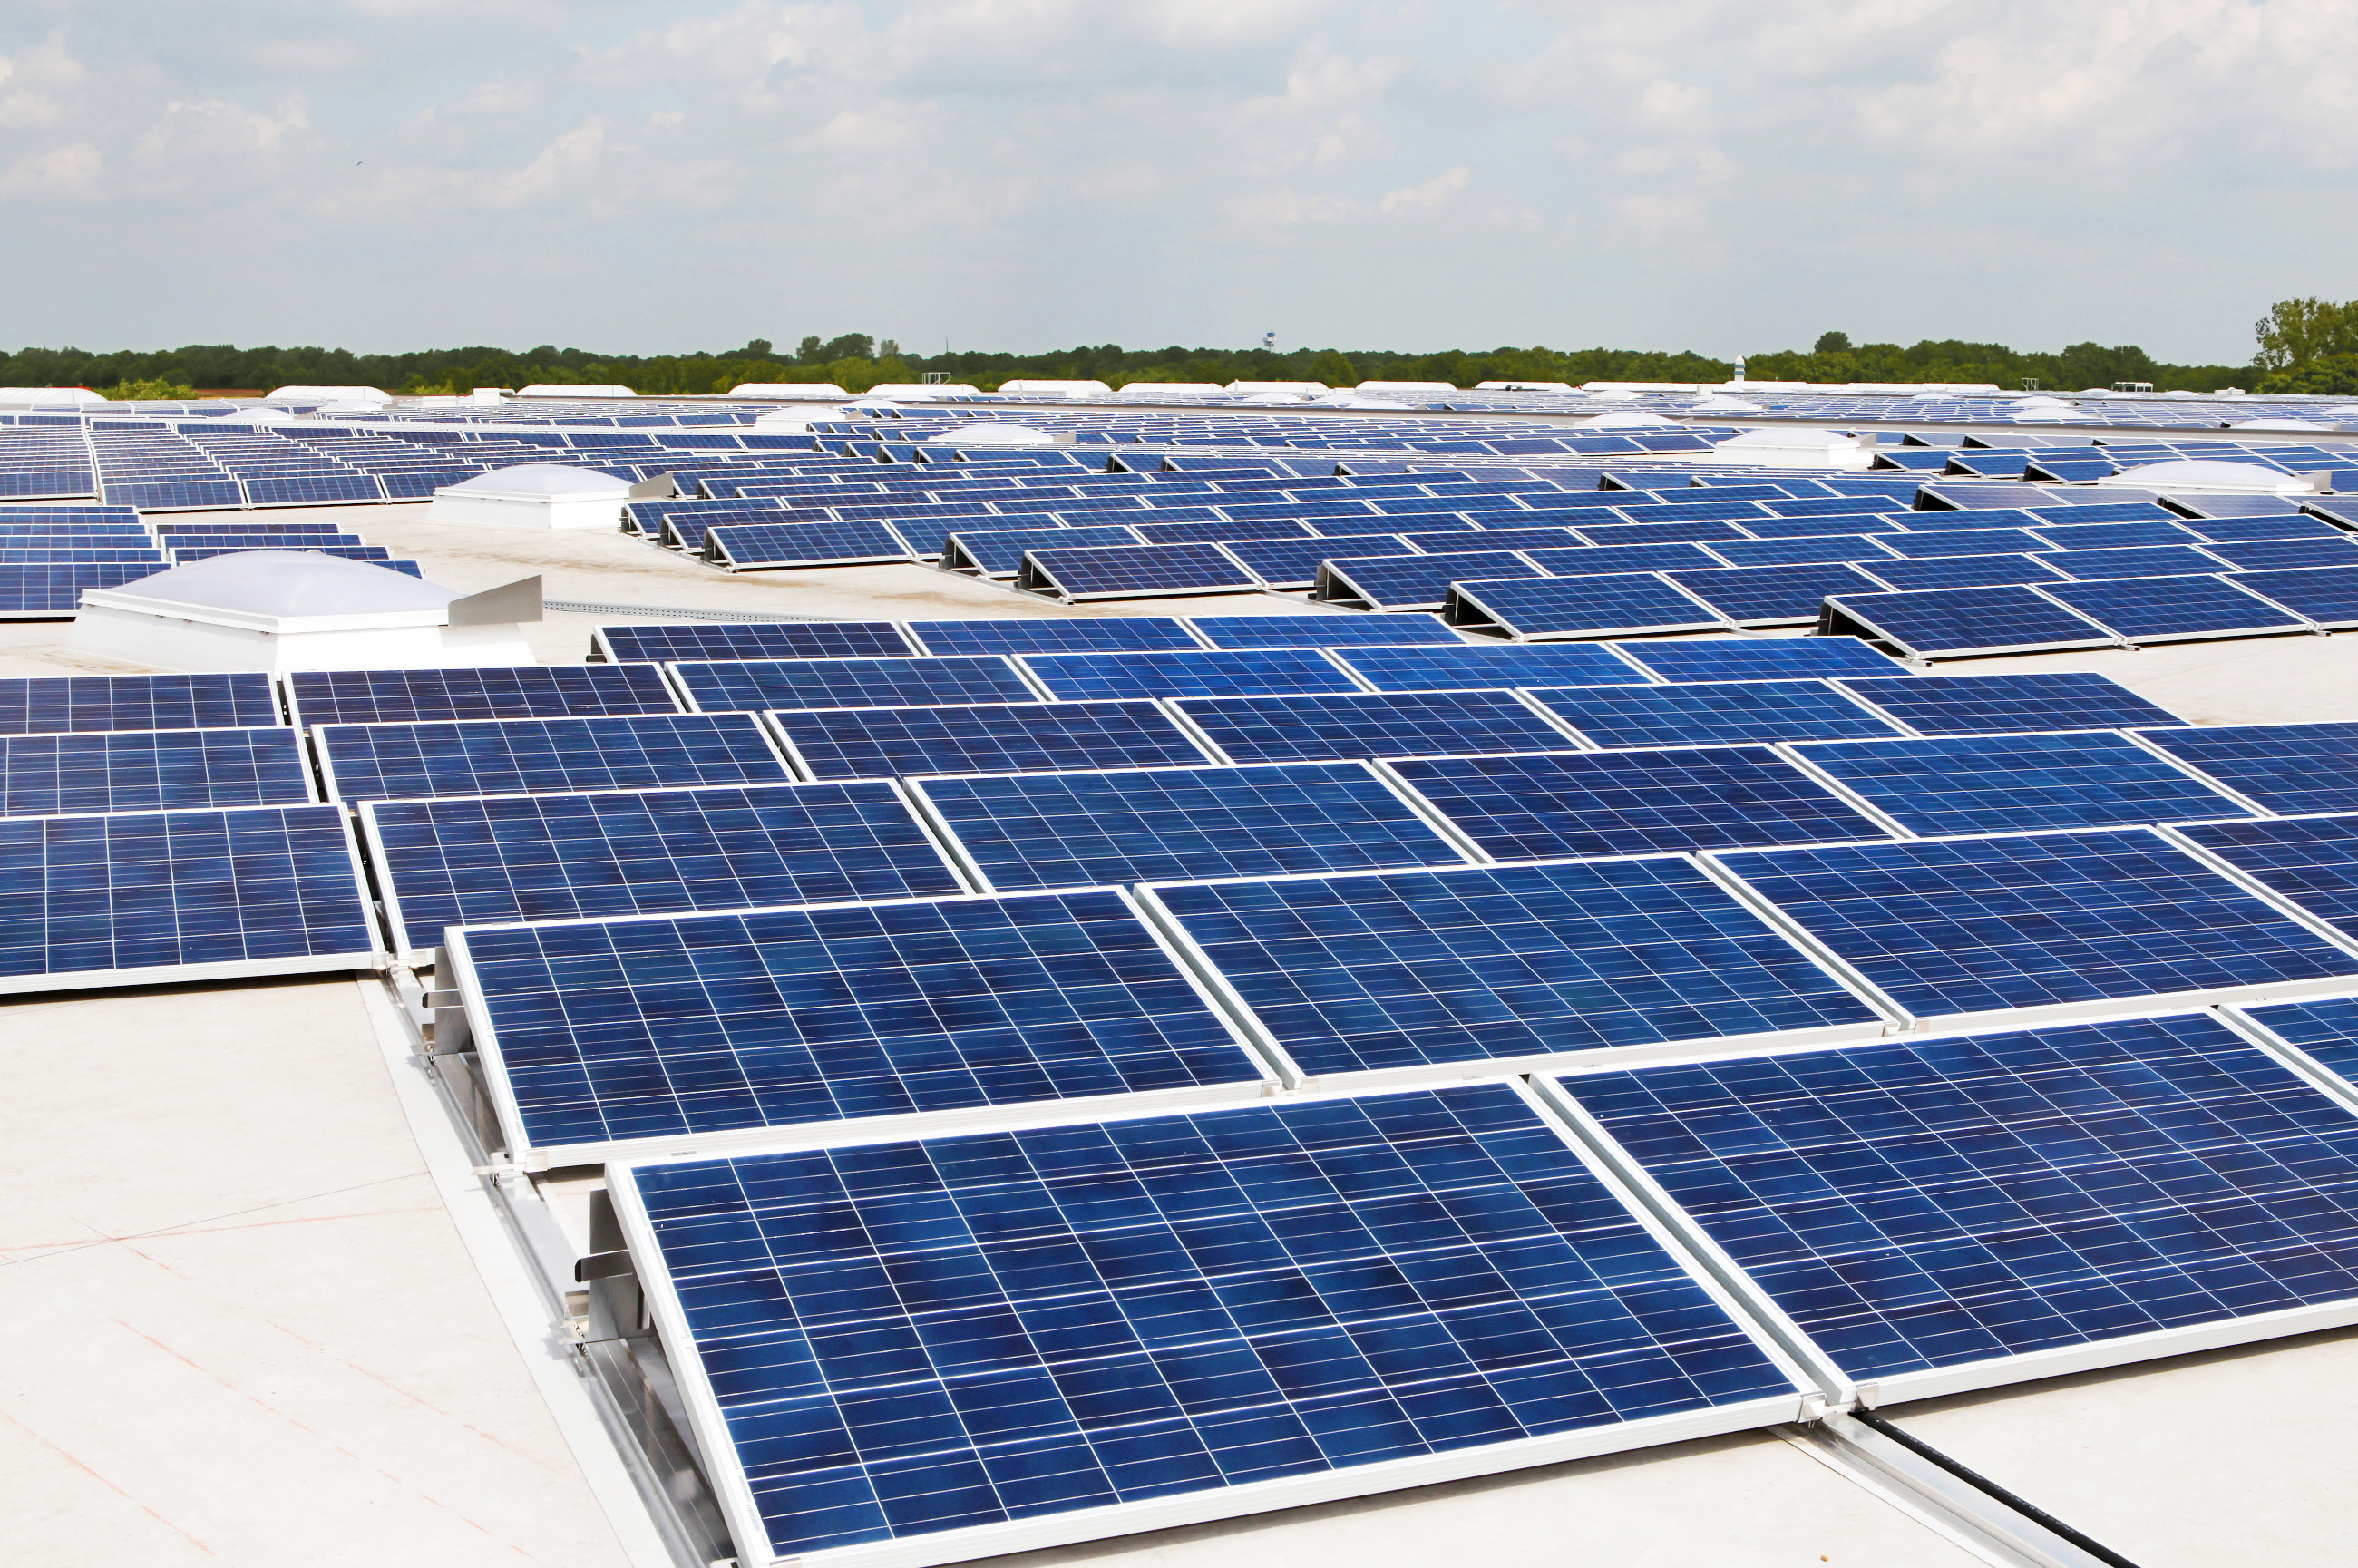
\includegraphics[width=\paperwidth,height=\paperheight]{images/titlepage/titlepic.jpg}%
        };

        % ------------------------------------------------ %
        % Info Table                                       %
        % ------------------------------------------------ %
        \node[%
            fill=black,
            fill opacity=0.75,
            rounded corners,
            outer sep=0pt,
            inner sep=1em,
            yshift=9em,
            anchor = south%
        ] at (current page.south) {\textcolor{white}{\infotable}};

        % ------------------------------------------------ %
        % FHNW Logo                                        %
        % ------------------------------------------------ %
        \node[anchor=north west,xshift=\logoX,yshift=-\logoY,outer sep=0pt,inner sep=0pt] at (current page.north west) {%
            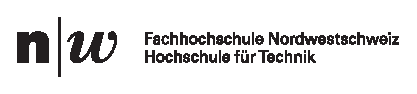
\includegraphics[height=12mm]{images/titlepage/fhnw.eps}%
        };
    \end{tikzpicture}



    % ---------------------------------------------------- %
    % The Text can  be set rather low in  the page without %
    % adjusting the top lengths.                           %
    % Backing up  and reseting these lengths  seems not to %
    % be necessary;  it appears  they are restored  at the %
    % end of the titlingpage environment.                  %
    % ---------------------------------------------------- %
    \setlength{\headsep}{0pt}
    \setlength{\headheight}{0pt}
    \setlength{\uppermargin}{4em}
    \checkandfixthelayout


    % ---------------------------------------------------- %
    % By   default,  centering   inside  the   titlingpage %
    % environment  will   center  with  respects   to  the %
    % typeblock. When  the  typeblock  is  centered,  this %
    % leads to  centered text  with respect to  the entire %
    % title  page. However,  When  the  typeblock  is  not %
    % centered, some adjustment is needed.                 %
    % See memman Chapter "Titles" for more information.    %
    % ---------------------------------------------------- %
    \calccentering{\unitlength}
    \begin{adjustwidth*}{\unitlength}{-\unitlength}


    % ---------------------------------------------------- %
    % Work some  magic to  automatically adjust  the hrule %
    % lengths to the length of the book title.             %
    %                                                      %
    % NOTE: The  font  size setting  needs  to  be in  the %
    % \mytitle  command, otherwise  \settolength will  not %
    % take it  into account  and will only  calculate with %
    % the default font size.                               %
    %                                                      %
    % NOTE  2: This mechanism  breaks if  the title  spans %
    % across multiple  lines. You're on  your own  in that %
    % case.                                                %
    % ---------------------------------------------------- %
    \newcommand{\mytitle}{{\textbf{\fontsize{25mm}{1em}\selectfont Project Powerline}}}
    \newlength{\titlelength}            % Length of title text
    \settowidth{\titlelength}{\mytitle}
    \newcommand{\titlerulefactor}{1.2}  % Length of title rules, as a factor

    % ---------------------------------------------------- %
    % Set the title color                                  %
    % ---------------------------------------------------- %
    \newcommand{\titlecolor}{black}

    % ---------------------------------------------------- %
    % Put the title onto the page                          %
    % ---------------------------------------------------- %
    \textcolor{\titlecolor}{%
        \centering
        \rule{\titlerulefactor\titlelength}{1pt} \\
        \vspace*{4mm}
        \mytitle\\
        %\vspace*{5mm}
        \rule{\titlerulefactor\titlelength}{1pt} \\
        \vspace*{6mm}
        \fontsize{8mm}{1em}\selectfont Fachbericht \\
    }


    % ---------------------------------------------------- %
    % This is the end of the centering magic.              %
    % ---------------------------------------------------- %
    \end{adjustwidth*}


    % ---------------------------------------------------- %
    % Make  sure  this  is   not  put  into  \frontmatter, %
    % otherwise it will get a \frontmatter folio.          %
    % \cleardoblepage  is not  actually necessary  because %
    % it  is  automatically   called  by  the  titlingpage %
    % environment.                                         %
    % ---------------------------------------------------- %
    %\cleardoublepage

    %\setlength{\headsep}{\originallength}
    %\checkandfixthelayout
\end{titlingpage}


% -------------------------------------------------------- %
% See  the  memoir  documentation  for  what  specifically %
% frontmatter does. Among  other things, page  numbers are %
% set to roman numerals and chapter numbers are removed.   %
% -------------------------------------------------------- %
\frontmatter

% -------------------------------------------------------- %
% Comment out what's not needed, obviously.                %
% -------------------------------------------------------- %
%\begin{centering}
\vspace*{30mm}
\begin{tiny}
    \begin{tabular}{lll}
        Inhalt & \copyright~2016 & Reto Nussbaumer   \\
               &                 &                   \\
        Design & \copyright~2016 & Raphael Frey      \\
    \end{tabular}


    % ---------------------------------------------------- %
    % Having  this  in  a  tabular  is  a  bit  ugly,  but %
    % it  ensures alignment  and  limited paragraph  width %
    % without much effort.                                 %
    % ---------------------------------------------------- %
    \vspace{1em}
    \begin{tabular}{p{.9\textwidth}}
        \noindent  Erstellt  im  Fr\"uhlingssemester 2016  an  der  Hochschule
        f\"ur  Technik  der  Fachhochschule   Nordwestschweiz  im  Rahmen  des
        Modules   \emph{Projekt  4}   des   Studiengangs  \emph{Elektro-   und
        Informationstechnologie}. \\

        \\
        \iftoggle{paper}{%
            Dies     ist    die     Druckversion    dieses     Dokuments. Eine
            elektronische     Version      mit     farbig     hervorgehobenen,
            klickbaren   Links   ist   auf  den   abgegebenen   elektronischen
            Datentr\"agern  in  Anhang \ref{app:electronicStorage}  auf  Seite
            \pageref{app:electronicStorage}   zu   finden    oder   kann   bei
            \code{raphael.frey@students.fhnw.ch} angefordert werden.
        }{%
            Dies ist die elektronische  Ausf\"uhrung des Dokuments. Links sind
            farbig hervorgehoben und klickbar. Falls eine Version ohne farbige
            Akzentuierung erw\"unscht ist, kann diese bei
            \href{mailto:raphael.frey@students.fhnw.ch}{\code{raphael.frey@students.fhnw.ch}}
            angefordert werden.
            % internet links: blau
            % externe links: magenta
        }
        \\

        \\
        Dieses Dokument hat bisher \thecounttexruns~Kompiliervorg\"ange durchlaufen. \\
    \end{tabular}
    \vspace{1em}

    \begin{tabular}{>{\ttfamily}lrl}
        Version 1 & 16.06.2016 & Abgabe \\
    \end{tabular}

    \vspace{1em}
    \begin{tabular}{l @{${}:{}$} l}
        Quelle Titelbild & \cite{ref:titlepage:pvanlage} \\
        Quelle Logo FHNW & \cite{ref:fhnwlogo}           \\
    \end{tabular}
\end{tiny}
%\\
%\footnotesize{\checkmark~\np~\noi~\partially} \\
%\\
%\large{\checkmark~\np~\noi~\partially} \\
%\\
%\checkmark~\np~\noi~\partially
%\end{centering}

% **************************************************************************** %
\chapter*{Management Summary}
\label{chap:mgmtsum}
% **************************************************************************** %

\section*{Main Ideas and facts}
For  Project 4  in the  spring  semester 2015  the students  were assigned  to
develop  an electro  mechanical system  to  keep a  laser pointer  steady. The
device should be able to emit a laser beam and keep it steady even if the user
is nervous and  trembling. The goal of this project is  to develop a prototype
that  is small  and  light enough  to  carry around  and  hold a  presentation
with. Another focus was on the budget: The  production costs of a series of 20
pieces should not exceed 120 CHF per unit.

\section*{Background}
In the autumn semester  2014, a group of students were  assigned with the task
to  find out  if  itwould be  possible  to develop  such  an anti-shake  laser
pointer, the results were inconclusive. Theparticipants agreed that the device
should be able to perform at a frequency range of 3 to 20 Hz.

\section*{Results}
The final prototype  did not meet the expectations. It is  able to correct low
frequency movements,but it struggles when  it is shaken at higher frequencies.
The prototype is small, it blends in with the usual laser pointers although it
is slightly  larger in  diameter. The estimated  price per  unit to  produce a
series  of 20  is around  70 SFr. However,  this figure  does not  include the
casing,  which was  produced for  free  by the  FHNW mechanical  workshop. The
prototype is powered by  a battery that is rechargeable by USB  and is able to
last eight hours.

\section*{Conclusions}
The approach of deflecting the laser beam with stepper motors seems promising,
the power usage is manageable and it allows a very small size, while the price
for the  parts is low. While the  overall concept and the  peripheral hardware
are solid and meet the expectations, there is the problem that the device does
not work at  higher frequencies.  The stepper motors used  in this project are
probably a  bit too cheap and  tend to break. A simulation  in Simulink showed
that the problem lies within  the laser deflection mechanism. We estimate that
the moment  of inertia  of the components  is too much  for the  small stepper
motors.

\section*{Recommendation}
To get rid of the flaws  in higher frequency performance, we suggest improving
the laser deflection mechanism. Most likely  reducing weight would not cut it,
as laser diodes can’t  get much smaller than the one  we use. This means the
whole  deflection  mechanism  should be  redesigned. Also,  different  stepper
motors should be considered.

%\include{frontmatter/dedication}
%\include{frontmatter/declaration}
%\include{frontmatter/acknowledgements}


% -------------------------------------------------------- %
% The starred versions do not make an entry for themselves %
% in the ToC, the unstarred versions do.                   %
% -------------------------------------------------------- %
\tableofcontents*
\newpage
%\listoffigures
%\listoftables


% -------------------------------------------------------- %
% Set page numbers to  arabic numerals, reset page counter %
% to 1, display  chapter numbers. See memoir documentation %
% for more information.                                    %
% -------------------------------------------------------- %
\mainmatter


% -------------------------------------------------------- %
% It is  advisable to use actually  meaningful chapter and %
% section names instead of generically numbered ones as in %
% this  example structure. That  way, their  place in  the %
% document is not directly tied to their file name, and it %
% is  possible to  restructure the  document (e.g.  move a %
% section  from one  chapter  to another,  or reorder  the %
% chapters)  without  needing  to adjust  file  names  and %
% similar shenanigans.                                     %
% -------------------------------------------------------- %
% **************************************************************************** %
\chapter{Einleitung}
\label{chap:einleitung}
% **************************************************************************** %

Photovoltaikanlagen   sind  heutzutage   kein   Nischenprodukt  mehr. Um   die
Abhängigkeit  vom Erdöl  zu verringern,  werden vielerorts  kleine, aber  auch
grosse  Anlagen gebaut. Die  W\"arme-Energie, welche  kostenlos von  der Sonne
kommt,  wird  in elektrische  Energie  umgewandelt  und  kann gleich  vor  Ort
genutzt werden. Anlagenbesitzer  investieren meistens einen grossen  Betrag in
eine  neue  Anlage  und  sind  darauf angewiesen,  dass  diese  den  maximalen
Ertrag  liefert. Das ist  in der  Regel  ohne grossen  Aufwand der  Fall. Doch
es  gibt Umstände,  welche  die Effizienz  einer Photovoltaikanlage  erheblich
verringern  können und  dies meist  ohne, dass  es jemand  bemerkt.  In  einer
Photovoltaikanlage  werden üblicherweise  mehrere  PV-Module  zu einem  String
zusammengefasst,  indem  sie  in   Serie  geschaltet  werden. Dabei  kann  ein
abgeschattetes,  verschmutztes  oder  gar  defektes  Modul  den  Strom  dieser
Serieschaltung und somit auch die Leistung des gesamten Strings und der Anlage
stark beeinträchtigen. Was grosse finanzielle Einbussen zur Folge haben kann.

Das  Ziel des  Projektes P4  war es,  ein PV-Überwachungssystem  bestehend aus
einer Sensorplatine für den Einbau in  die Anschlussbox jedes Moduls und einem
zentralen Meldegerät  für den Einbau  im Schaltschrank beim  Wechselrichter zu
entwickeln, aufzubauen und zu testen. Die  Sensorplatine soll die Spannung des
jeweiligen PV-Modules  messen und sie  an das Mastergerät über  die bestehende
DC-Leitung  der  Anlage  übermitteln. Im  Mastergerät  werden  die  gemessenen
Spannungen der  einzelnen PV-Module  gespeichert und  ausgewertet. Erkennt das
Mastergerät ein fehlerhaftes  PV-Modul, soll eine Alarmierung  am Gerät selbst
und  per  SMS  ausgegeben  werden. Zusätzlich wird  ein  Relais  zur  externen
Signalisation  betätigt.   Das  System  soll  möglichst  energieeffizient  und
kostengünstig sein,  um die wirtschaftlichkeit einer  Photovoltaikanlage nicht
zu verschlechtern.

Das  Hauptproblem liegt  bei  der Signalübertragung  über  die DC-Leitung  der
Photovoltaikanlage. Denn die Spannung darauf schwankt  zwischen 12 und 60 Volt
an der Sensorplatine  und beträgt am Mastergerät bis zu  1000 Volt. Auf dieser
Leitung  ein Signal  zu  übertragen  ist schwierig  und  wird heutzutage  kaum
gemacht.  Zudem muss auf kleine Leistung beim gesamten System geachtet werden,
um keine wertfolle Energie zu verschwenden.

\todo{Beschreibung unseres Produkts}

Der vorliegende  Bericht stellt  die technische Dokumentation  unseres Systems
dar.  Zuerst wird das Konzept unserer L\"osung beschrieben, zusammen mit einer
Benutzerf\"uhrung.  Anschliessend  wird auf  das Hardware-  und Firmwaredesign
eingegangen,  und   zuletzt  werden  die  am   System  durchgef\"uhrten  Tests
dokumentiert.

\lipsum

% **************************************************************************** %
\chapter{Markante Ereignisse}
\label{chap:markant}
% **************************************************************************** %

Das  Ishikawa-Diagramm   in  Abbildung  \ref{fig:ursache:wirkung}   auf  Seite
\pageref{fig:ursache:wirkung}  stellt  die   drei  wichtigsten  positiven  und
negativen Erfahrungen dar, welche im Verlauf des Projektes gemacht wurden. Die
meisten  dieser   Erfahrungen  wurden   im  Bereich  Projektarbeit   und  Team
Zusammenarbeit gemacht. Die technische Herausforderung  des Projekts 4 war vom
Modul gegeben. Es  wurden erstmals  alle erlernten  Methoden und  Theorien bei
einem Projekt verwendet, wobei die F\"ahigkeiten aller Teammitglieder zu sehen
waren.

Zu  Beginn  des  Projektes  wurden  sehr  schnell  Fortschritte  erzielt,  wie
zum  Beispiel die  Fertigstellung  des ersten  Sensorplatinen-Prototypen. Dies
stimmte das  gesamte Team optimistisch,  dass wir unser  Projektziel erreichen
k\"onnten. Dies war zu  Beginn alles andere als  klar. Die Zusammensetzung aus
drei ETH  Abg\"angern und  drei berufsbegleitend Studierenden,  welche jeweils
nur wenig Projekt- und Elektronikerfahrung  hatten, liess ein sehr schwieriges
Projekt erahnen. Trotz  dieser schwierigen Voraussetzungen war  das ganze Team
sehr motiviert und auch bereit ein hochwertiges Produkt zu entwickeln.

Die beste  positive Erfahrung wurde  bei der Zusammenarbeit  gemacht. Das Team
konnte kaum unterschiedlicher sein. Dies hatte  jedoch keinen Einfluss auf die
Arbeitsmoral  der Mitglieder. Alle  gaben  ihr Bestes  und  jeder konnte  sein
K\"onnen unter  Beweis stellen. Was  unter dem  st\"andigen Stress  im Projekt
keine Selbstverst\"andlichkeit  darstellt. Ebenfalls eine sehr  gute Erfahrung
wurde beim Arbeiten  am Fachbericht gemacht. Der Dokumentationsverantwortliche
hatte  gl\"ucklicherweise   bereits  einige  Erfahrungen  mit   Schreiben  von
Berichten. Dadurch  lief  die  Planung  der  Dokumentation  sehr  planm\"assig
und  ohne  nennenswerte Verz\"ogerungen. Er  konnte  die  einzelnen Teile  gut
zusammenf\"uhren und  ermahnte alle  Teammitglieder regelm\"assig,  ihren Teil
beizutragen.

Es wurden  jedoch auch negative Erfahrungen  gemacht, welche vor allem  in der
zweiten Projekth\"alfte auftraten. Die  Softwareentwicklung wurde planm\"assig
in dieser  Zeit begonnen und  war bereits  nach zwei Wochen  in Verzug. Leider
konnte dieser  Verzug w\"ahrend  mehreren Wochen  nicht behoben  werden, trotz
starker  Bem\"uhungen  vom  halben   Team. Ein  st\"andiges  Problem  war  die
Zuverl\"assigkeit  einiger  Teammitglieder. Es  kam   einige  Male  vor,  dass
zugeteilte Aufgaben nicht wie  erwartet erledigt wurden. Dieses Problem konnte
gl\"ucklicherweise bis zum Projektende behoben werden.

{\begin{a3pages}
    \begin{tikzpicture}[remember picture,overlay]
        \node at (current page.center) {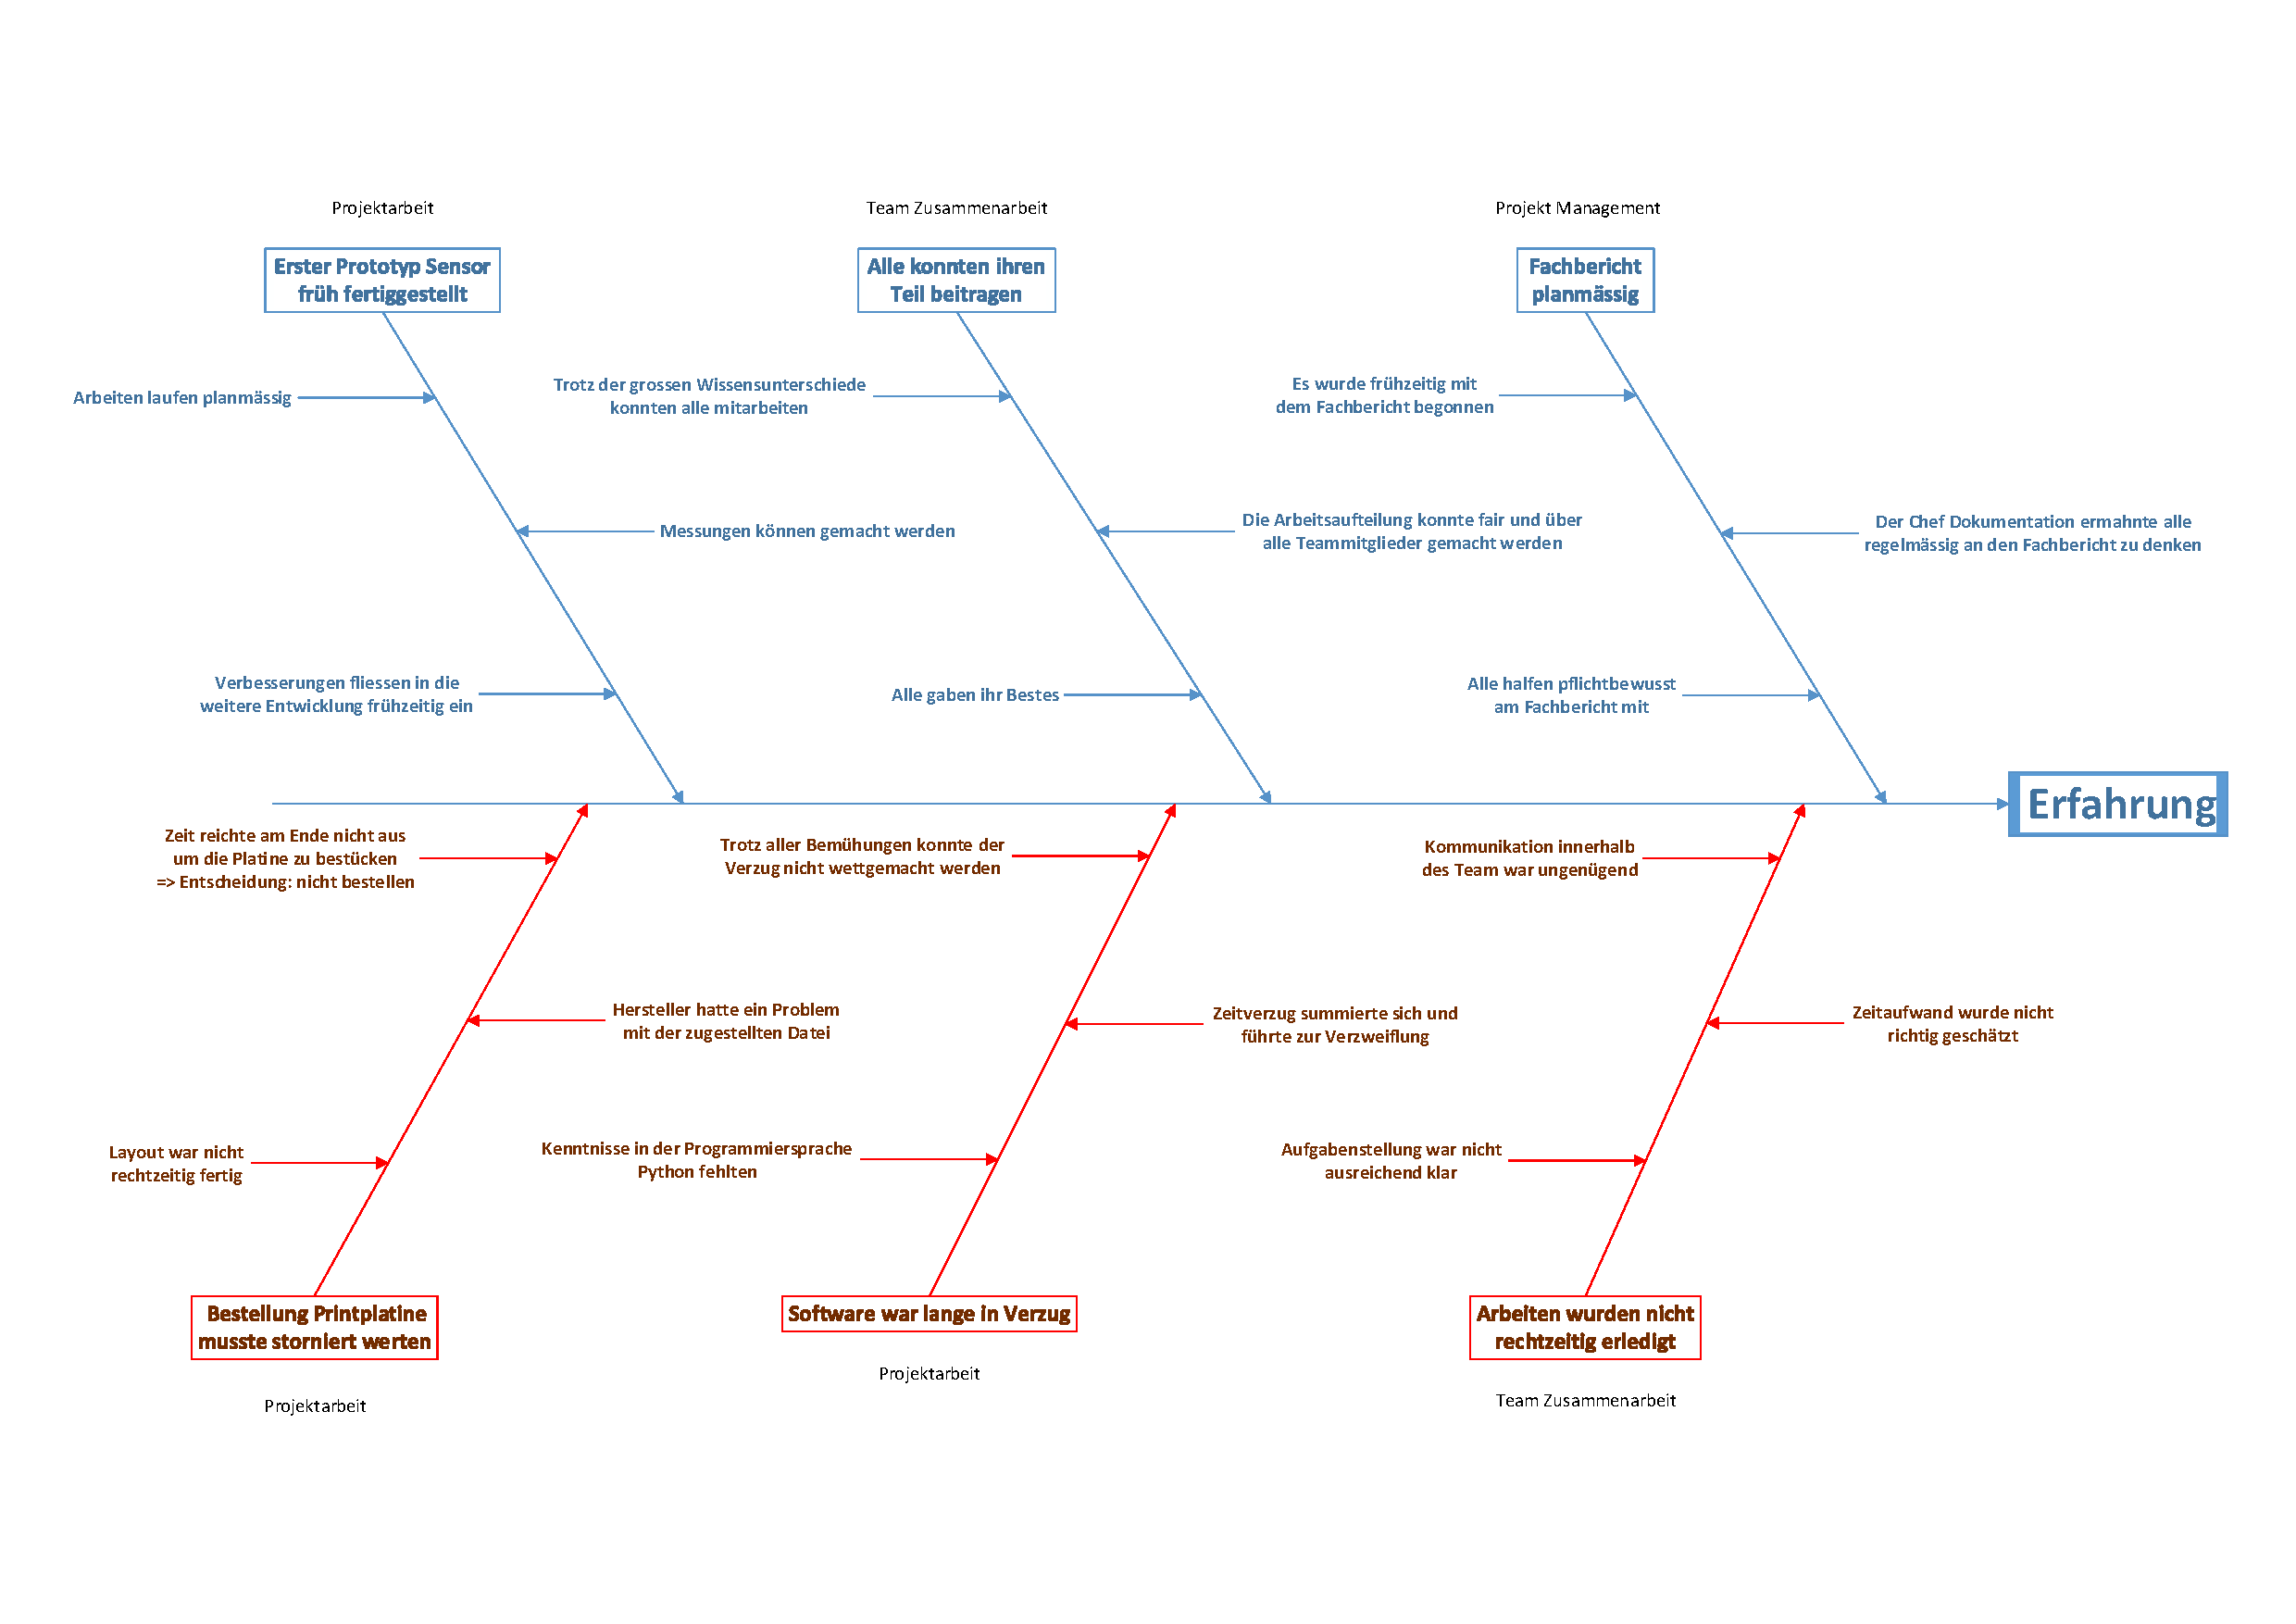
\includegraphics[width=0.85\paperwidth]{images/ursache-wirkung.pdf}};
    \end{tikzpicture}
    \vspace*{202mm}
    \figcaption{Ursache-Wirkung-Diagramm f\"ur unser Projekt}
    \label{fig:ursache:wirkung}
\end{a3pages}}

% **************************************************************************** %
\chapter{Reflexion}
\label{chap:reflexion}
% **************************************************************************** %

In diesem Kapitel werden von den  zuvor genannten Ereignissen je zwei negative
und  zwei  positive  Punkte  reflektiert. Die einzelnen  Reflexionen  sind  in
Abschnitte  gegliedert,  die zuerst  die  Ausgangslage  und anschliessend  die
Planabweichung  erl\"autert. Folgend werden  Massnahmen  und deren  Auswirkung
genannt. Am Schluss  wird ein Fazit  gezogen, um die gemachten  Erfahrungen im
n\"achsten Projekt verbessern zu k\"onnen.

% ---------------------------------------------------------------------------- %
\section{Erster Prototyp Sensor fr\"uh fertiggestellt}
\label{sec:firstSensorprototype}
% ---------------------------------------------------------------------------- %

Am  Anfang des  Projektes war  eine grosse  Unsicherheit vorhanden,  dass kein
Hardware-Teil entstehen  w\"urde, denn  im Team befand  sich nur  ein Mitglied
mit  Hardware-Erfahrung. Die  Motivation  war  dementsprechend  klein  und  es
musste  nach  einer  L\"osung  gesucht  werden. Nach  einer  Sitzung  mit  der
Projektbetreuerin  konnte  eine  L\"osung  f\"ur  die  fehlende  Erfahrung  im
Bereich  Hardware gefunden  werden. Das Team  erhielt noch  ein zus\"atzliches
Mitglied, welches \"uber die n\"otige  Erfahrung verf\"ugte.  Damit war bereit
ein  fr\"uhes Ereignis  erfolgreich  behandelt worden. Denn  der Zeitplan  war
\"ausserst ehrgeizig kalkuliert.

Gem\"ass   Planung  wurde   erwartet,  dass   beide  Hardware-Teile   (Sensor-
und    Masterplatine)    bis    zur   Projektwoche    fertiggestellt    werden
k\"onnten. Anschliessend  sollte   die  Validierung  und   die  dazugeh\"orige
Software  erarbeitet  werden. Mit  diesem   Zeitplan  war  gen\"ugend  Reserve
eingerechnet um allf\"allige Probleme aufzufangen.

Dank  der  guten  Arbeit  des  Hardware-Teams wurde  der  erste  Prototyp  der
Sensorplatine noch vor dem  geplanten Zeitpunkt fertiggestellt. Das ermunterte
das ganze  Team und zeigte, dass  etwas erreicht werden konnte  mit gen\"ugend
Einsatz.

Dank der M\"oglichkeit  die Sensorplatine in einem  privaten Bastelraum selbst
herzustellen,  konnte  rund  eine Woche  Wartezeit  weggelassen  werden. Diese
Wartezeit w\"are  entstanden, wenn das  Printed Circuit Board (PCB)  bei einem
Hersteller im Ausland hergestellt worden w\"are. So konnte dieses Arbeitspaket
viel fr\"uher als erwartet abgeschlossen werden.

F\"ur   folgende   Projekte  soll   mitgenommen   werden,   dass  nach   allen
M\"oglichkeiten  gesucht werden  soll, um  Zeit einzusparen. Die  Zeit ist  im
Projekt  die  knappste Ressource  und  meistens  liegt  ein Scheitern  an  der
Zeitknappheit.

% ---------------------------------------------------------------------------- %
\section{Fachbericht planm\"assig}
\label{sec:reportAsPlanned}
% ---------------------------------------------------------------------------- %

Der  Fachbericht ist  beim  Projekt  4 ein  zentrales  Element, welches  stark
gewichtet wird. Aus diesem Grund war  es wichtig den Fachbericht w\"ahrend dem
gesamten Projekt  immer im Hinterkopf  zu behalten. Die Erfahrung  zeigt, dass
der Fachbericht  immer in letzter Minute  fertig gestellt wird oder  sogar nur
einen Teil seiner zwingenden Inhalte besitzt.

Im  Team   wurde  f\"ur   diese  wichtige   Aufgabe  ein   Chef  Dokumentation
ernannt. Damit  konnte  sichergestellt  werden,  dass eine  Person  f\"ur  den
Bericht   verantwortlich  war. Die   Planung  der   Dokumentation  konnte   so
zuverl\"assig  erstellt  werden  und   allf\"allige  Probleme  wurden  schnell
erkannt.   Die  zust\"andige  Person  war   sehr  kompetent  und  mahnte  alle
Teammitglieder regelm\"assig,  ihre Teile  vom Fachbericht rechtzeitig  und in
geforderter Qualit\"at zusammenzustellen.

Das Resultat  dieses Vorgehens war  schnell zu sehen. Der Fachbericht  nahm ab
der Projektwoche Formen an, was gem\"ass Planung zu erwarten war. So kam keine
Hektik  beim Schreiben  auf und  ein qualitativ  hochwertiges Dokument  konnte
zusammengestellt werden. Es war zum Projektende \"ubersichtlich, vollst\"andig
und vor allem sch\"on anzusehen.

Der  Fachbericht  ist   bei  jedem  Projekt  ein   zentrales  Element. In  ihm
werden  alle wichtigen  Erkenntnisse zusammengefasst. Ebenfalls  enth\"alt der
Fachbericht  auch  alle  Entscheidungen,   welche  im  Verlauf  des  Projektes
getroffen wurden. So kann nachvollzogen werden, welche Entscheidungen zum Ziel
f\"uhrten und welche nicht. Im Falle eines  Scheiterns kann das Projekt ab der
letzten  richtigen  Entscheidung  fortgesetzt  und doch  noch  zu  einem  Ziel
gef\"uhrt  werden. Darum war  die  Entscheidung, einen  Chef Dokumentation  zu
ernennen,  richtig und  sollte bei  weiteren Projekten  auf jeden  Fall wieder
getroffen werden.

% ---------------------------------------------------------------------------- %
\section{Bestellung der Printplatine muss storniert werden}
\label{sec:orderCancelled}
% ---------------------------------------------------------------------------- %

Das  Ereignis  trat  in  der  drittletzten Woche  des  Semesters  auf. Es  war
beabsichtigt  worden die  finalen Platinen  bei einem  Platinen Hersteller  zu
bestellen,  damit professionelle  Platinen  best\"uckt werden  konnten. Leider
wurde schlussendlich  entschieden, diese  Bestellung nicht  auszul\"osen, weil
die  verbleibende  Zeit   nicht  ausgereicht  h\"atte,  um   die  Platinen  zu
best\"ucken und zu testen.

Es  war  geplant,  die  zwei  Platinen  vom  Sensor  und  vom  Master  in  der
zehnten Semesterwoche  zu bestellen. Damit  h\"atte die Zeit  ausgereicht alle
Bauelemente auf die Platine zu  l\"oten und anschliessend ausf\"uhrliche Tests
durchzuf\"uhren. Dieses  Vorhaben verz\"ogerte  sich  um zwei  Wochen, da  der
Zeitaufwand f\"ur das Platinen-Design h\"oher als erwartet war.

Die Abweichung vom  Zeitplan waren zu sp\"at  erkannt worden. Das Arbeitspaket
Platinen-Layout war einerseits  zu knapp bemessen, was auf  Grund der geringen
Projekterfahrung  des Teams  zur\"uckzuf\"uhren  war. Zus\"atzlich wurde  erst
am  eigentliche  Bestelldatum  darauf  aufmerksam gemacht,  dass  die  Platine
noch  nicht  fertig  designt  worden   war,  um  bestellt  zu  werden. Nachdem
rund  eineinhalb  Wochen  sp\"ater  als geplant  das  Design  fertig  gestellt
wurde, wurde  die Bestellung  via Ansprechperson  f\"ur Bestellungen  der FHNW
ausgel\"ost. Leider wurde vom  Hersteller mitgeteilt, dass es  ein Problem mit
der  zugestellten Datei  gab. Diese Mitteilung  wurde im  Team nicht  nach der
Vereinbarung der internen Kommunikation weitergegeben, sodass ein weiterer Tag
verging bis etwas unternommen werden konnte. Zu diesem Zeitpunkt war das halbe
Hardwareteam unerwartet  krank, was eine schnelle  L\"osung verhinderte. Durch
das  gemeinsame Auftreten  der  verschiedenen Probleme,  musste eine  radikale
Entscheidung  getroffen werden. Im  Plenum wurden  schlussendlich Entschieden,
dass   die  Bestellung   der  Platinen   storniert  wird. Damit   konnte  eine
\"Uberbelastung des  Hardware-Teams in  den letzten  Semesterwochen verhindert
werden und der Fokus konnte auf die \"ubrigen Aufgaben gelegt werden.

Dank  dieser Entscheidung  konnten  alle  verbleibenden Arbeiten  sorgf\"altig
erledigt werden. Es wurde  nicht auf Kosten anderer  Arbeiten ein halbherziges
Produkt zusammengebastelt. Die Entscheidung war auf jeden Fall richtig. Da sie
vom ganzen  Team unterst\"utzt  wurde, arbeiteten  alle motiviert  weiter, was
nicht  selbstverst\"andlich war. Es  wurden viele  Stunden in  das Design  der
Platinen investiert, welche leider nicht hergestellt werden konnten.

Was bleibt  ist die Erfahrung,  wie in solchen Situationen  vorgegangen werden
soll. Tritt  ein  kleines  Problem  auf, kann  meist  eine  schnelle  L\"osung
gefunden werden. Treten jedoch mehrere  gravierende Probleme am gleichen Punkt
auf und  herrscht zus\"atzlich  Zeitnot, so  ist eine  gesamthafte Beurteilung
gefragt. Die L\"osung  muss auf jeden  Fall realisierbar sein und  darf keinen
negativen Einfluss auf andere Arbeiten  haben. Nicht, dass am Ende das gesamte
Projekt  in Mitleidenschaft  gezogen wird,  weil  nur ein  kleiner Teil  nicht
planm\"assig funktioniert.


% ---------------------------------------------------------------------------- %
\section{Software lange im Verzug}
\label{sec:softwareBehind}
% ---------------------------------------------------------------------------- %

Der Softwareteil  war lange  Zeit in Verzug. Die  einzelnen Teile  waren nicht
rechtzeitig fertiggestellt worden und oder nur mangelhaft funktionsf\"ahig. Es
konnte  festgestellt  werden,  dass   nicht  gen\"ugend  Fachwissen  vorhanden
war. Wie im  Risikomanagement aufgef\"uhrt, waren die  Auswirkungen erheblich.
Viele folgende Arbeiten verz\"ogerten sich oder konnten nicht erledigt werden.

Urspr\"unglich  waren  die  Arbeiten  an der  Software  vor  der  Projektwoche
geplant. Auf  Antrag  des  gesamten  Teams  wurden  die  Softwarearbeiten  auf
die  Projektwoche   und  die   darauffolgenden  Wochen   verschoben. Denn  die
Evaluation  der Bauelemente,  respektive des  Mikrocontrollers war  noch nicht
abgeschlossen. Dieser  war   die  Basis  der   Software. Diese  Plan\"anderung
war  kurz  nach  Beginn  des  Projektes  entstanden  und  zu  jenem  Zeitpunkt
zu  verantworten. Leider  konnten die  Arbeiten  nicht  in gew\"unschter  Zeit
abgeschlossen  werden, welches  zwar  fr\"uhzeitig erkannt  wurde, aber  nicht
behoben werden konnte.

Die   Ursache  dieses   Ereignisses   ist  auf   den   Anfang  des   Projektes
zur\"uckzuf\"uhren. Es wurde am Anfang  definiert welche Komponenten verwendet
werden und in welcher Programmiersprache die einzelnen Teilsysteme geschrieben
werden. Durch  die  grosse  Erfahrung  von  zwei  Teammitglieder  mit  Python,
wurde diese  Programmiersprache f\"ur  das Masterger\"at  gew\"ahlt. Zudem war
ein  Raspberry Pi  als  zentrales Element  f\"ur  das Masterger\"at  gew\"ahlt
worden,  aus  den  gleichen  Gr\"unden  wie  die  Programmiersprache. Es  soll
erw\"ahnt werden,  dass auf Raspberry  Pi die  Sprache Python sehr  einfach zu
implementieren war. Diese Entscheidung war zu dieser Zeit einleuchtend. Leider
musste  schnell  festgestellt werden,  dass  es  sehr zeitintensiv  war,  eine
komplett neue Programmiersprache zu  erlernen und damit ein funktionsf\"ahiges
Programm zu schreiben.

Die  fehlende  Erfahrung  konnte  nur schwer  behoben  werden. Die  erfahrenen
Mitglieder hatten auch ihre eigenen  Arbeiten zu erledigen und waren ebenfalls
unter Zeitdruck. Dadurch entstand eine immer gr\"osser werdende Verz\"ogerung,
die  nur  mit  sehr  viel   Zeitaufwand  der  Beteiligten  verkleinert  werden
konnte. Dies  ben\"otigte unn\"otig  viel Zeit  und h\"atte  verhindert werden
k\"onnen.

Als  Erfahrung   f\"ur  das  n\"achste   Projekt  soll  auf   bekannte  Mittel
zur\"uckgegriffen werden. Es  wird viel  zu viel  Zeit ben\"otigt  neue Mittel
(z.B.  eine  neue Programmiersprache,  ein  neues  Programm usw.)  ausreichend
effizient  zu verwenden. Bekanntes  aus  dem Unterricht  ist  meist mit  wenig
Aufwand wieder verf\"ugbar und vor allem kann einfach beim Fachdozenten um Rat
gefragt werden. Die Idee  vom Projekt ist es, das erlernte  Anzuwenden und bei
Unklarheiten nachzufragen. Es soll nicht das Rad neu erfunden werden, denn das
ist enorm zeitintensiv.

% **************************************************************************** %
\chapter{Schlusswort}
\label{chap:schlusswort}
% **************************************************************************** %

Leider  konnte  kein   funktionierender  Prototyp  entwickelt  werden. Daf\"ur
wurden  einige Teilsysteme  fertiggestellt. Die gr\"osste  Herausforderung war
wohl  die  \"Ubertragung  der  Messdaten  \"uber  die  Gleichstromleitung  der
Photovoltaikanlage. Diese konnte  getestet werden und funktionierte  sehr gut,
was  sehr erfreulich  war. Zudem wurde  das Masterger\"at  in einem  Geh\"ause
untergebracht, wobei die Men\"uf\"uhrung  voll funktionierte. Ein Prototyp der
Sensorplatine war ebenfalls  funktionsf\"ahig und zu all dem  waren auch viele
Simulationen sehr erfolgsversprechend.

Im   Projektmanagement   wurden   einige   Fehleinsch\"atzungen   gemacht. Zum
Beispiel   fehlten  getrennte   Arbeitspakete  f\"ur   die  Sensor-   und  die
Masterplatine. Weiter  wurde  der  Arbeitsaufwand bei  einigen  Arbeitspaketen
untersch\"atzt. Denn  obwohl  die  ganze  Planung in  der  Gruppe  detailliert
besprochen   wurde,   konnten   die  Fehleinsch\"atzungen   nicht   korrigiert
werden. Dies ist  ganz klar  auf die  mangelnde Projekterfahrung  des gesamten
Teams  zur\"uckzuf\"uhren. Positiv   zu  erw\"ahnen  ist,  dass   das  gesamte
Projektmanagement  mit allen  Elementen  konsequent  durchgef\"uhrt wurde  und
auch  Erfolge mit  sich brachte. Es  konnten einige  organisatorische Probleme
wie  zum  Beispiel  unklare Aufgabenstellungen,  Zust\"andigkeitsprobleme  und
zwischenmenschliche Konflikte mit den gelernten Methoden entsch\"arft werden.

Die wichtigste  Erfahrung \"uber das  ganze Projekt war, dass  auf Bew\"ahrtes
gesetzt  werden   sollte.   R\"uckblickend   war  es  illusorisch   f\"ur  das
Projekt  eine  unbekannte  Programmiersprache,  ein  neues  Layout-Tool,  neue
Mikrocontroller zu  verwende und alles  im kleinstm\"oglichen Format  bauen zu
wollen.   All diese  neuen Teile  f\"uhrten zu  einem enormen  Zeitaufwand und
schlussendlich zu einem nicht funktionierenden Prototyp.

Es  wurden jedoch  auch  sehr positive  Erfahrungen  gemacht. Obwohl das  Team
kaum  unterschiedlicher sein  konnte, wurde  sehr fleissig  und zielorientiert
zusammengearbeitet. Die  fertigen   Teile  des   Projektes  waren   von  guter
Qualit\"at und jedes Mitglied konnte sein Bestes dazu beitragen.



% -------------------------------------------------------- %
% Appendices are  usually numbered  and therefore  part of %
% the mainmatter, not the backmatter.                      %
% The advice about meaningful chapter names applies to the %
% appendices as well, see above.                           %
% -------------------------------------------------------- %
%\appendixpage
%\appendix
%% **************************************************************************** %
\chapter{Parameter des Solarzellenmodells}
\label{app:celldata}
% **************************************************************************** %

Zur  Herleitung  der  Zellenparameter  werden vier  Quellen  herangezogen,  um
ein  einigermassen  gut  abgest\"utztes Ergebnis  zu  erhalten. Die  gesuchten
Parameter sollen  f\"ur am Markt  erh\"altliche Module g\"ultig  sein, weshalb
Datenbl\"atter von Solar\emph{modulen} und nicht Zellen verwendet werden.

Zuerst  werden  Zellenstrom  und Zellenspannung  bestimmt,  anschliessend  die
Fl\"ache einer Zelle,  um damit auf die im Modell  verwendete Kapazit\"at, den
Shunt-Widerstand und den Seriewiderstand schliessen zu k\"onnen.


% ---------------------------------------------------------------------------- %
\section{Zellenstrom und Zellenspannung}
\label{app:sec:cell:UI}
% ---------------------------------------------------------------------------- %

Tabelle   \ref{tab:moduleData:IU}    auf   Seite   \pageref{tab:moduleData:IU}
enth\"alt die  Daten zu  Kurzschlussstr\"omen und Leerlaufspannungen  von vier
Modulen. Die  Spannung  $U_{\mathrm{OC,  Zelle}}$ pro  Zelle  (letzte  Spalte)
errechnet sich gem\"ass:

\begin{equation}
    \label{eq:voltagePerCell}
    U_{\mathrm{OC, Zelle}} = \frac{U_{\mathrm{OC, Strang}}}{\text{Anzahl Zellen pro Strang}}
\end{equation}

\begin{table}
    \centering
    \small
    \caption{%
        Daten   f\"ur   Solarmodule.  \textbf{pk}:   polykristallines   Panel,
        \textbf{mk}:     monokristallines     Panel.     \emph{Anmerkung}: Die
        Konfiguration  der Module  (wieviele  Zellen in  Serie  und wie  viele
        Str\"ange  parallel)  ist  mit   Ausnahme  des  Solarex  MSX-60  nicht
        angegeben. Es  ist  aber  bekannt,  in  welcher  Gr\"ossenordnung  die
        Spannung  pro  Zelle  ungef\"ahr  liegen sollte,  womit  man  aus  den
        angegebenen  Leerlaufspannungen  und  der Gesamtzahl  Zellen  auf  die
        Konfiguration eines Modules schliessen kann.%
    }
    \label{tab:moduleData:IU}
    \begin{tabular}{lp{20mm}lllll}
        \toprule
          \rotatebox{70}{\pbox{25mm}{Quelle}}
        & \rotatebox{70}{\pbox{25mm}{Modell}}
        & \rotatebox{70}{\pbox{25mm}{Kurzschluss-\\strom $I_{\mathrm{SC}}$}}
        & \rotatebox{70}{\pbox{25mm}{Leerlauf-\\spannung $V_{\mathrm{OC}}$}}
        & \rotatebox{70}{\pbox{25mm}{Anzahl Zellen \\(total)}}
        & \rotatebox{70}{\pbox{25mm}{Anzahl Zellen \\(Strang)}}
        & \rotatebox{70}{\pbox{25mm}{Leerlaufspan-\\nung pro Zelle}} \\
        \midrule

          \cite{ref:solar:bonkoungou}
        & Solarex MSX-60
        & \SI{3.8}{\ampere}
        & \SI{21.1}{\volt}
        & \num{36}
        & \num{36}
        & \SI{586}{\milli\volt}
        \\

          \cite{ref:solar:px85}
        & Sunset PX85 (\textbf{pk})
        & \SI{5.5}{\ampere}
        & \SI{21.5}{\volt}
        & \num{76}
        & \num{38}
        & \SI{566}{\milli\volt}
        \\

          \cite{ref:solar:as150}
        & Sunset Solargenerator AS150 (\textbf{mk})
        & \SI{8.7}{\ampere}
        & \SI{22.3}{\volt}
        & \num{36}
        & \num{36}
        & \SI{620}{\milli\volt}
        \\

          \cite{ref:solar:sunmodulePro}
        & Sunmodule Pro-Series XL SW320 (\textbf{mk})
        & \SI{9.41}{\ampere}
        & \SI{45.9}{\volt}
        & \num{72}
        & \num{72}
        & \SI{638}{\milli\volt}
        \\

        \bottomrule
    \end{tabular}
\end{table}

Wir verwenden f\"ur  die Simulation einer Zelle den  gerundeten Mittelwert der
Zellenspannungen aus der letzten Spalte von Tabelle \ref{tab:moduleData:IU}:

\begin{equation}
    \label{eq:cell:UOC}
    \underline{\underline{U_{\mathrm{OC, Zelle, Simu}} = \SI{600}{\milli\volt}}}
\end{equation}

Polykristalline  Zellen  liefern  bedeutend  kleinere  Kurzschlusstr\"ome  als
monokristalline  Zellen.  Jedoch  werden bei  monokristallinen Zellen  weniger
Str\"ange parallel  geschaltet, womit  der Gesamtstrom  des Moduls  immer noch
unter \SI{10}{\ampere}  bleibt. Unabh\"angig vom  genauen Aufbau  eines Moduls
gehen wir  daher davon aus,  dass es  nicht mehr als  \SI{10}{\ampere} liefern
wird.


% ---------------------------------------------------------------------------- %
\section{Bestimmung der Zellenfl\"ache}
\label{app:sec:cell:surface}
% ---------------------------------------------------------------------------- %

Das    PX-85-Modul   aus    \cite{ref:solar:px85}    verwendet   76    Zellen,
angeordnet  in   einer  $4  \times  19$   -  Konfiguration. Seine  Abmessungen
betragen   $\SI{1477}{\milli\meter}    \times   \SI{660}{\milli\meter}$,   was
sich   herunterrechnen  l\"asst   auf  eine   ungef\"ahre  Modulgr\"osse   von
$\SI{165}{\milli\meter}   \times   \SI{75}{\milli\meter}$. Dabei  werden   die
Abmessungen   des   Rahmens   und   die  Abst\"ande   zwischen   den   Modulen
vernachl\"assigt.

Die Fl\"ache  des AS-150-Moduls wird analog  aus Quelle~\cite{ref:solar:as150}
zu  $\SI{155}{\milli\meter}  \times   \SI{164}{\milli\meter}$  bestimmt.   Das
XL-320-Modul   aus   \cite{ref:solar:sunmodulePro}    hat   die   Zellgr\"osse
direkt    angegeben,    sie     betr\"agt    $\SI{156}{\milli\meter}    \times
\SI{156}{\milli\meter}$. Es ist naheliegend dass aufgrund von Standardisierung
das AS-150-Modul die gleiche Zelldimension hat wie das XL-320-Modul, n\"amlich
den verbreiteten 6-Zoll-Formfaktor.

Da  eine gr\"ossere  Zelle eine  gr\"ossere Kapazit\"at  und somit  gr\"ossere
Probleme   im  Falle   der  Kurzschlussvariante   bedeutet,  wird   mit  einer
Zellgr\"osse   von   $\SI{156}{\milli\meter}  \times   \SI{156}{\milli\meter}$
gerechnet, womit sich die Fl\"ache der Zelle bestimmt zu:

\begin{equation}
    \label{eq:cell:surface}
    \underline{\underline{A_{\mathrm{Zelle}} = \SI{156}{\milli\meter} \times \SI{156}{\milli\meter} = \SI{243.36}{\centi\meter\squared}}}
\end{equation}

Dies     entspricht     ungef\"ahr     der     600-fachen     Fl\"ache     des
\SI{0.43}{\centi\meter\squared}-Modules aus  Quelle \cite{ref:solar:scofield}.



% -------------------------------------------------------- %
% Page  numbering continues,  but chapter  numbers are  no %
% longer  displayed. See  memoir  documentation  for  more %
% information.                                             %
% -------------------------------------------------------- %
\backmatter

% -------------------------------------------------------- %
% Bibliography: We  are using  the  IEEEtran package  from %
% Michael Shell                                            %
%                                                          %
% There  are  a  few  different  styles  in  the  IEEEtran %
% package.   We are  going to  use  one of  two of  those, %
% either in the sorted or unsorted variety.                %
%                                                          %
% The sorted  version sorts  bibliographic entries  in the %
% bibliography alphabetically, while  the unsorted version %
% lists bibliographic  entries in the order  in which they %
% were cited (first occurrence).                           %
% -------------------------------------------------------- %
%\bibliographystyle{bibliography/IEEEtranS} % sorted
\raggedright
\bibliographystyle{bibliography/IEEEtran} % unsorted
\bibliography{bibliography/references}
\end{document}
